%\documentclass[11pt,handout]{beamer}
\documentclass{beamer}
\usepackage[ngerman]{babel}
\usepackage[utf8]{inputenc}
\usepackage{amsmath}
\usepackage{amssymb}
\usepackage{listings} 
\usepackage{stmaryrd}
\lstset{language=Python, tabsize=4, showstringspaces=false,basicstyle=\footnotesize,mathescape=true} 
\lstset{literate=%
  {Ö}{{\"O}}1
  {Ä}{{\"A}}1
  {Ü}{{\"U}}1
  {ß}{{\ss}}1
  {ü}{{\"u}}1
  {ä}{{\"a}}1
  {ö}{{\"o}}1
}
\usepackage{mathtools}
\usepackage{ulem}
\usepackage{tikz}

\usetheme{Boadilla}
\mode<presentation>{
\useoutertheme[subsection=false]{miniframes}
\useinnertheme{rectangles}
%\usecolortheme{crane}
}
\parskip 10pt



\begin{document}
\title{Informatik}   
\author{Rekursion} 
\date{}
\frame{\titlepage} 

%---
\begin{frame}[fragile]
Eine Funktion darf sich im Rumpf selbst wieder aufrufen. 
Man nennt das einen rekursiven Aufruf. \pause Jede Rekursion braucht eine Bremse,
 damit es nicht zu unendlich vielen Aufrufen kommt. \pause 

Iterative Definition der Fakultät: \pause

$n! =\begin{cases}
 1   &  n = 0 \\
 1 \cdot 2 \cdot 3 \cdot ... \cdot n & n > 0 
\end{cases} $ \pause 

Rekursive Definition der Fakultät: 

$n! =\begin{cases}
 1   & n = 0 \\ 
 (n-1)! \cdot n & n > 0 
\end{cases} $
\end{frame}


%---
\begin{frame}[fragile]
\begin{lstlisting} 
# iterative Implementation der Fakultät
def fakultaet(n):
    if n $==$ 0: return 1
    temp = 1
    for i in range(n):
        temp = temp * (i+1)
    return temp

# rekursive Implementation der Fakultät
def fakultaet(n):
    if n $==$ 0: return 1
    return n * fakultaet(n-1)
    
#Aufruf:
print(fakultaet(5))
\end{lstlisting} 
\end{frame}


%---
\begin{frame}[fragile]

Iterative Definition der Zweierpotenz:

$2^n =\begin{cases}
 1   &  n = 0 \\
 2 \cdot 2 \cdot 2 \cdot ... \cdot 2 \text{  (n-mal)} & n > 0 
\end{cases} $ \pause

Rekursive Definition der Zweierpotenz:

$2^n =\begin{cases}
 1,   & n = 0 \\
 2^{n-1} \cdot 2 & n > 0 
\end{cases} $
\end{frame}


\begin{frame}[fragile]
Eine rekursive Methode darf die Lösung für \textit{kleinere Problemgrößen} in ihrem Rumpf benutzen. \pause

Die Methode dreheUm dreht die Reihenfolge der Zeichen eines Strings um. \pause
\begin{lstlisting} 
def dreheUm(s):
    if len(s) $==$ 0:
        return ''
    letztes = s[-1]
    bisVorletztes = s[:-1]
    return letztes + dreheUm(bisVorletztes)

Aufruf:
print(dreheUm("Python"))
\end{lstlisting} 
\end{frame}

\begin{frame}[fragile]
Türme von Hanoi

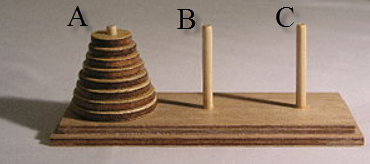
\includegraphics[scale=0.6]{Hanoi.png} \pause

Der Turm soll von Position A nach Position C. Die Scheiben dürfen nur einzeln bewegt werden und nie darf eine größere auf eine kleinere Scheibe gelegt werden. Eine Zwischenposition B steht zur Verfügung. 

https://www.youtube.com/watch?v=w9LgLiW9YHU \pause

Rekursive Idee: verlagere den Turm ohne die unterste Scheibe rekursiv nach B (kleinere Problemgrößen dürfen wir als
gelöst annehmen). Verlege dann die unterste Scheibe von A nach C und verlagere dann den kleineren Turm rekursiv von B nach C.
\end{frame}

\begin{frame}[fragile]
\begin{lstlisting} 
def hanoi(n, start, ziel, zwischen):
    if n $==$ 0: return
    hanoi(n-1,start,zwischen,ziel)
    print("Scheibe",n," von ",start," nach ",ziel)
    hanoi(n-1,zwischen,ziel,start)
    
Aufruf:
hanoi(5,"A","C","B")
\end{lstlisting} 
\end{frame}

\begin{frame}[fragile]
\begin{minipage}[t]{6cm}
\begin{tabular}{ll}
Scheiben & Verlegeoperationen\\
1  &  1 \\   \pause
2 &  3  \\
3 &   7 \\
4 & 15 \\
5 & 31 \\
6 & 63 \\
n &  \pause $2^n-1$  
\end{tabular}
\end{minipage}  \pause
\begin{minipage}[t]{5cm}
1 Verlegeoperation = \\
1 Sekunde 

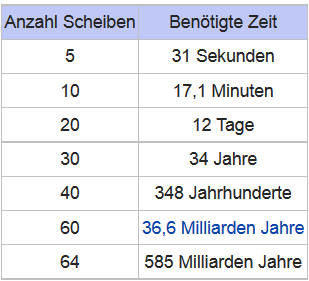
\includegraphics[scale=0.7]{Hanoi2.png}
\end{minipage}


\end{frame}

%----
\begin{frame}[fragile]

Fibonacci-Zahlen

\begin{tabular}{|c|c|c|c|c|c|c|c|c|c|}
\hline n  & 1 & 2 & 3 & 4 & 5 & 6 & 7 & 8 &...\\
\hline fib(n)  & 1 & 1 & 2 & 3 & 5 & 8 & 13 & 21 & ...\\
\hline
\end{tabular} \pause

Rekursive Definition der Fibonacci-Zahlen:

$fib(n) =\begin{cases}
 1   &  n \le 2 \\
 fib(n-1) + fib(n-2) & n > 2 
\end{cases} $ \pause

\begin{lstlisting} 
# Fibonacci-Zahlen rekursiv
def fib(n):
    if n <= 2: return 1
    return fib(n-2) + fib(n-1)
\end{lstlisting} \pause

Schon fib(40) dauert ziemlich lange.
\end{frame}

%----
\begin{frame}[fragile]

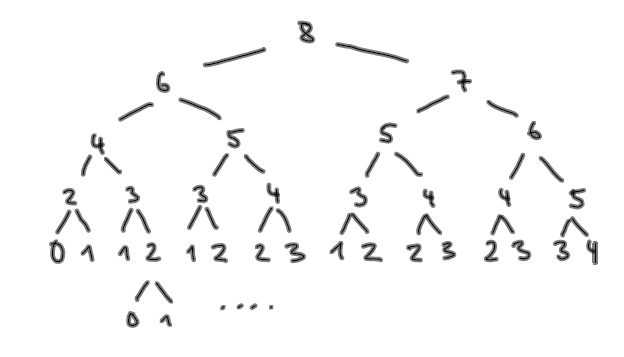
\includegraphics[scale=0.7]{fib.png} \pause

Rekursive Implementation ist sehr unwirtschaftlich, da schnell anwachsende Zahl von fib-Aufrufen.

\end{frame}

%----
\begin{frame}[fragile]
Besser: \textit{dynamische Programmierung} = Tabellen mit Teillösungen aufbauen. \pause

%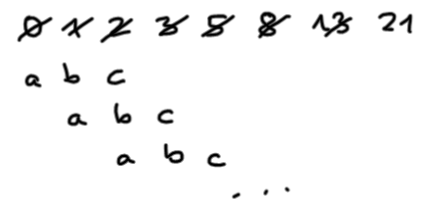
\includegraphics[scale=0.5]{fib2.png} \pause
\begin{lstlisting} 
def fib(n):
    if n <= 2: return 1
    a,b = 1,1
    for i in range(3,n+1):
        c = a+b
        a,b = b,c
    return c
\end{lstlisting} 

\end{frame}



\end{document}